%{Förkunskaper: mängder, heltalsdivision, potenser}
\chapter{Talsystem}\index{talsystem}\index{talbeteckningssystem|see{talsystem}}
\label{ch:Talsystem}
\lettrine{V}{i vet sedan} tidigare avsnitt att tal existerar och att det finns
olika typer av tal; naturliga tal, hela tal, rationella tal och irrationella
tal.
Vi vet dessutom att det finns oändligt\footnote{Med detta är det inte sagt att
de olika mängderna har samma kardinalitet.} många tal av varje typ samt att de
går att räkna med på olika sätt.
Men vad är egentligen ett tal?

Ett tal är inom matematiken ett \emph{abstrakt objekt} som följer givna regler,
som vi sett i kapitlen om de naturliga (\cref{DeNaturligaTalen}) och de hela 
talen (\cref{ch:Heltalen}).
Är då \(123\) ett tal?
Nej, som framgått av vår tidigare redogörelse för talen är \(123\) bara en 
\emph{representation} av talet vi \emph{benämner} etthundratjugotre.
Etthundratjugotre är följaktligen också enbart en representation av talet.

Ett talsystem\index{talsystem}, eller
talbeteckningssystem\index{talbeteckningssystem}, tillhandahåller ett entydigt
sätt att representera dessa abstrakta tal på.
Detta görs genom olika tecken och teckenkombinationer.
De tecken vi är vana vid i västkulturerna är siffrorna \(0\) till \(9\), vilka 
ursprungligen är arabiska siffror.
Vi behöver här skilja på ett tal och en siffra.
Siffror är tecken som används för att representera tal.
Det vill säga, talet \(123\) representeras av sammansättningen av de tre
siffrorna \(1,2\) och \(3\).

Genom historien har det använts många olika talsystem, varav några finns kvar
än idag.
I \cref{tbl:OlikaEtthundratjugotre} ges några representationer av
etthundratjugotre i olika talsystem.

\begin{table}
  \caption{%
    Olika representationer av etthundratjugotre i olika talsystem.
  }\label{tbl:OlikaEtthundratjugotre}
  \begin{tabular}{ll}
    \toprule
    Binära talsystemet & \(1111011\) \\
    Decimala talsystemet & \(123\) \\
    Hexadecimala talsystemet & \(7B\) \\
    Romerska talsystemet & CXXIII \\
    \bottomrule
  \end{tabular}
\end{table}

\begin{exercise}\label{xrc:HittaTalsystem}
  Lista alla sätt du känner till att representera tal på.
\end{exercise}
\begin{exercise}\label{xrc:SkapaTalsystem}
  Hitta på ett eget sätt att representera tal på.
\end{exercise}

Det talsystem som är vanligast idag är det \emph{decimala talsystemet}, där
tecknen som används är siffrorna \(0, 1, 2, 3, 4, 5, 6, 7, 8\) och \(9\).
\begin{remark}
  Märk väl skillnaden mellan ett decimalt tal och ett tal angivet med decimal.
  Ett decimalt tal är ett tal representerat med det decimala talsystemet.
  Det andra är ett tal med decimalkomma och decimaler, exempelvis
  \(1.2\).
\end{remark}
Andra vanliga talsystem är det binära, med siffrorna \(0\) och \(1\), och det
hexadecimala, med 16 olika siffror.
Dessa två används flitigt inom datateknik.
Det decimala, det binära och det hexadecimala talsystemen är av en speciell
typ av talsystem som kallas \emph{positionssystem}.
Anledningen till namnet är att en siffras position har betydelse för dess
värde.
\begin{example}\label{ex:PositionensBetydelse}
  I \(111\) betyder den första ettan \(100\) medan den andra ettan
  betyder \(10\) och den sista betyder \(1\).
  Det vill säga, samma siffra har olika betydelse beroende på vilken position
  den har i representationen som den befinner sig i.
\end{example}
Positionssystemen behandlas i detalj i ett kommande avsnitt.

Det romerska talsystemet är däremot inte ett positionssystem, utan är en
modifikation av typen \emph{teckenvärdessystem}.
Det romerska systemet behandlas i nästa avsnitt.


%%%%%%%%%%%%%%%%%%%%%%%%%%%%%%%%%%%%%%%%%
% DET ROMERSKA TALSYSTEMET
%%%%%%%%%%%%%%%%%%%%%%%%%%%%%%%%%%%%%%%%%
\section{Det romerska talsystemet}
\index{romerska talsystemet}\index{talsystem!romerskt}
\label{sec:RomerskaTalsystemet}
Det romerska talsystemet är baserat på en modifikation av ett
\emph{teckenvärdessystem}.
I ett teckenvärdessystem har varje tecken ett speciellt värde.
Detta till skillnad från positionssystemet där positionen är avgörande för
tecknets värde.
I ett mycket enkelt teckenvärdessystem, som används idag, representerar ett
streck talet ett, två streck representerar talet två, och så vidare till och
med talet fyra.
Det vill säga, samma tecken har alltid samma värde och upprepningar adderas
tillsammans för att få talet de representerar.
Talet fem representeras däremot med fyra streck, som ovan, och ett femte streck
snett över de fyra andra strecken.
Detta bildar ett nytt tecken även om det är logiskt uppbyggt från tidigare
tecken.
Systemet består således av två tecken, ett tecken som har värdet ett och ett
tecken som har värdet fem.
Se \cref{fig:Strecktal}.

\begin{figure}
  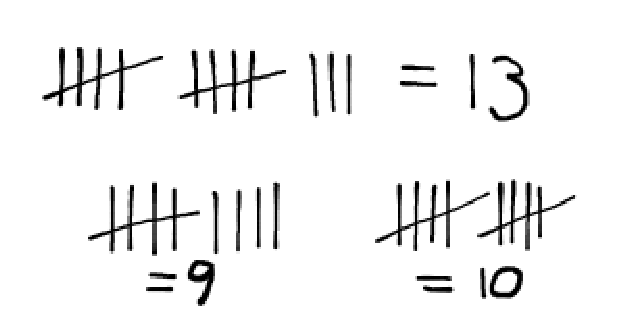
\includegraphics[width=4cm]{figs/strecktal.eps}
  \caption{%
    Tecknen i ett enkelt teckenvärdessystem.
  }\label{fig:Strecktal}
\end{figure}

Det romerska systemet är en modifiering av detta system.
Tecknen och deras betydelse i det romerska talsystemet ges i
\cref{tbl:RomerskaSiffror}.

\begin{table}
  \caption{%
    De romerska siffrorna.
  }\label{tbl:RomerskaSiffror}
  \begin{tabular}{ccccccc}
    \toprule
    I & V & X & L & C & D & M \\
    1 & 5 & 10 & 50 & 100 & 500 & 1000 \\
    \bottomrule
  \end{tabular}
\end{table}

Det romerska talsystemt fungerar nästan på samma sätt som ett
tecken\-värdes\-system.
Den väsentliga skillnaden är att i teckenvärdessystemet summeras alla tecknens
värden medan det i det romerska systemet även finns subtraktion.
I det romerska systemet subtraheras ett tecken av lägre värde som står före ett
tecken med högre värde.
Exempelvis, IV ger \(4\) eftersom att en etta står före en femma.
VI ger däremot \(6\) eftersom att tecknens värde summeras.
Talen 1-10 ges i \cref{tbl:RomerskaTal} och några andra större tal finns i
\cref{tbl:RomerskaTal2}.

\begin{table}
  \caption{%
    Talen 1-10 i det decimala och det romerska talsystemen.
  }\label{tbl:RomerskaTal}
  \begin{tabular}{lllllllllll}
    \toprule
    Decimala talsystemet & 1 & 2 & 3 & 4 & 5 & 6 & 7 & 8 & 9 & 10 \\
    Romerska talsystemt & I & II & III & IV & V &
      VI & VII & VIII & IX & X \\
    \bottomrule
  \end{tabular}
\end{table}

\begin{table}
  \caption{%
    Några tal skrivna med det romerska talsystemet.
  }\label{tbl:RomerskaTal2}
  \begin{tabular}{lll}
    \toprule
    \(2011\) & MMXI & \(1000+1000+10+1\) \\
    \(1999\) & MCMXCIX & \(1000+(1000-100)+(100-10)+(10-1)\) \\
    \(1998\) & MCMXCVIII & \(1000+(1000-100)+(100-10)+5+1+1+1\) \\
    \(587\) & DLXXXVII & \(500+50+10+10+10+5+1+1\) \\
    \(487\) & CDLXXXVII & \((500-100)+50+10+10+10+5+1+1\) \\
    \bottomrule
  \end{tabular}
\end{table}

Som kan ses i \cref{tbl:RomerskaTal2} är det eftersträvansvärt att så få
tecken som möjligt används vid subtraktion.
Exempelvis kan tänkas att \(487\) är \(500\) minus \(13\) och därför skulle
kunna skrivas som XIIID.\@
Det blir dock enklare att se om man istället använder C, eller \(100\), för
subtraktionen av D, eller \(500\), och sedan lägger till tecknen för \(87\)
som vanligt.

\begin{exercise}\label{xrc:RaknaMedRomerskaTal}
  Undersök och diskutera hur enkelt det är att räkna med och
  representera tal med det romerska talsystemet.
\end{exercise}
\begin{exercise}
  Med utgångspunkt i föregående övning, hur tror du att romarna bidragit till
  matematikhistorien?
\end{exercise}
\begin{exercise}
  Hur är det med talet noll och negativa tal i det romerska talsystemet?
\end{exercise}



%%%%%%%%%%%%%%%%%%%%%%%%%%%%%%%%%%%%%%%%%
% POSITIONSSYSTEM
%%%%%%%%%%%%%%%%%%%%%%%%%%%%%%%%%%%%%%%%%
\section{Positionssystem}
\index{positionssystem}\index{talsystem!positionssystem}
\label{sec:Positionssystem}
Som nämnts tidigare innebär ett positionssystem att samma tecken
har olika betydelse eller värde beroende på vilken position tecknet innehar.
Systemet har en \emph{talbas}.
Det decimala talsystemet har basen \(10\) och varje position motsvarar en
unik \(10\)-potens.
Siffran på denna position ger koefficienten för denna potens.

\begin{example}\label{ex:DecimaltPosistionssystem}
  Det decimala talsystemet har basen \(10\).
  Talet etthundratjugotre representeras i detta system som \(123\).
  Vi har då
  \[1\cdot10^2 + 2\cdot10^1 + 3\cdot10^0 = 100 + 20 + 3 = 123.\]
\end{example}
\begin{example}\label{ex:BinartPositionssystem}
  Det binära talsystemet har basen \(2\).
  Således representeras talet etthundratjugotre som \(1111011\).
  Vi har då
  \[1\cdot2^6 + 1\cdot2^5 + 1\cdot 2^4 + 1\cdot2^3 + 0\cdot2^2 +
  1\cdot2^1 + 1\cdot2^0 = 123.\]
\end{example}
\begin{example}
  Om ett positionssystem har basen \(b\) används då \(b\) antal siffror,
  dessa har värdena \(0, 1, 2, \ldots, b-1\).
  För att representera ett tal används summor av \(b\)-potenser där siffrans
  position avgör exponenten.
  Siffrans värde avgör koefficienten för, det vill säga hur många av, den
  specifika \(b\)-potensen som ska adderas.
  Det vill säga talet vars värde beräknas som
  \[
    d_1 b^{n-1} + d_2 b^{n-1} + \cdots + d_{n-1} b^1 + d_n b^0
  \]
  representeras som \(d_1d_2\cdots d_n\) i basen \(b\).
\end{example}

Det finns även andra talsystem, exempelvis babyloniernas
sexagesimala positionssystem\index{talsystem!babylonskt}
\index{talsystem!sexagesimalt} som hade basen \(60\).
Spår av detta kan vi idag se i hur vi räknar tid, att en minut har 60
sekunder och en timme har 60 minuter.
Vi använder dock inte 60 olika tecken för att representera våra sekunder och
minuter utan tar istället hjälp av det decimala talsystemet.
Det babylonska sexagesimalsystemet är det äldsta kända användandet av ett
positionssystem och härstammar från Babylonien\footnote{Babylonien låg i
södra delen av Mesopotamien, ungefär i dagens Irak.} omkring 3100 f.v.t.\  
\cite{Kline1990mtf1}.

Kan då alla naturliga tal verkligen representeras med en godtycklig bas på
detta sätt?
Följande sats visar att sådant är fallet.
\begin{theorem}\label{thm:PositionssystemAllaUnika}
  Låt \(b>1\) vara ett naturligt tal större än ett.
  För varje naturligt tal \(x\in\N\) existerar ett naturligt tal \(n>0\)
  strikt större än noll och naturliga tal \(d_i<b\), där \(1\leq i\leq n\),
  strikt mindre än \(b\) sådana att \(x\) kan skrivas som
  \begin{equation*}
    x = d_1 b^{n-1} + d_2 b^{n-2} + \cdots + d_{n-1} b^1 + d_n b^0.
  \end{equation*}
  Denna presentation är unik upp till ordningen av termerna.
\end{theorem}
För att kunna bevisa detta behöver vi först följande lemma.
\begin{lemma}\label{lem:NollEndastOmLika}
  Låt \(b>0\) vara ett naturligt tal större än noll, \(m\) och \(n\)
  naturliga tal och \(c=c_1b^{n-1}+c_2b^{n-2}+\cdots+c_{n-1}b+c_n\), där
  \(0<c_1<b\) och \(0\leq c_i<b\) för \(i=2,3,\ldots,n\), och
  \(d=d_1b^{m-1}+d_2b^{m-2}+\cdots+d_{m-1}b+d_m\), där \(0<d_1<b\) och \(0\leq
  d_j<b\) för \(j=2,3,\ldots,m\).
  Då gäller att \(c-d=0\) endast om \(n=m\) och \(c_i=d_i\) för
  \(i=1,2,3,\ldots,n\).
\end{lemma}
\begin{proof}
  Låt oss anta att \(n=m+k\) för något naturligt tal \(k\).
  Vi har då att
  \begin{equation*}
    c-d=c_1b^{n-1}+\cdots+c_{k-1}b^{n-k+1}+(c_k-d_0)b^m+\cdots+(c_n-d_m) =
    0.
  \end{equation*}
  Men \(c_1b^{n-1}\neq 0\) och då måste \(n=m\).

  Då har vi att
  \begin{equation*}
    c-d = (c_1-d_1)b^{n-1}+\cdots+(c_{n-1}-d_{n-1})b+(c_n-d_n) = 0.
  \end{equation*}
  Låt oss anta att \(c_n-d_n\neq 0\), om inte delar vi med \(b\) tills att vi
  får en nollskild term utan en faktor \(b\).
  Då får vi att
  \begin{equation}
    \label{eq:NollEndastOmLika}
    (c_0-d_0)b^n+\cdots+(c_{n-1}-d_{n-1})b = -(c_n-d_n).
  \end{equation}
  Eftersom att vänsterledet i \cref{eq:NollEndastOmLika} är delbart med
  \(b\) måste även högerledet vara detta eftersom att de är lika.
  Men eftersom att \(c_i<b\) och \(d_i<b\) har vi att
  \(-b<c_i-d_i<b\) för \(i=0,1,2,\ldots,n\).
  Då är \(-(c_n-d_n)\) delbar med \(b\) endast om \(-(c_n-d_n)=0\), vilket
  är en motsägelse.
  Då måste alla termer \(c_i-d_i=0\) för \(i=1,2,3,\ldots,n\).
\end{proof}

Nu är vi redo att visa satsen.
\begin{proof}[Bevis \cref{thm:PositionssystemAllaUnika}]
  Vi börjar med att visa att summan existerar.
  Om vi delar \(x\) med \(b\) får vi en kvot \(q_1\) och en restterm
  \(r_1\) sådana att \(x=q_1b+r_1\) och \(0\leq r_1<b\).
  Om vi på samma vis delar \(q_1\) med \(b\) får vi en kvot \(q_2\) och en
  restterm \(r_2\) sådana att \(q_1=q_2b+r_2\) och \(0\leq r_2 < b\).
  Upprepas detta förfarande får vi att \(q_i=q_{i+1}b+r_{i+1}\), \(i\in\N\).
  Från \cref{xrc:KvotenMindre} har vi att \(q_{i+1}<q_i\) eftersom att
  \(b>1\).
  Vi får då från välordningsprincipen för de naturliga talen att \(q_n=0\)
  för något \(n\in\N\).
  Vi nu sätter ihop dessa resultat enligt följande idé.
  Vi hade först att \(x=q_1b+r_1\), men \(q_1=q_2b+r_2\) och följaktligen är
  \[x=(q_2b+r_2)b+r_1.\]
  Eftersom att \(q_i=q_{i+1}b+r_{i+1}\) får vi att
  \begin{align*}
    x &= ((((q_n b + r_n) b + r_{n-1}) b + \cdots + r_3) b + r_2) b + r_1 \\
     &= r_n b^{n-1} + r_{n-1} b^{n-2} + \cdots + r_3 b^2 + r_2 b^1 + r_1 b^0.
  \end{align*}
  Om vi låter \(d_1=r_n, d_2=r_{n-1}, \ldots, d_{n-1}=r_2, d_n=r_1\) ser vi
  att vi får en summa på korrekt form.

  Antag att det för ett naturligt tal \(x\) finns två olika representationer
  \(c_1c_2\cdots c_n\) och \(d_1d_2\cdots d_m\), båda med basen \(b\).
  Detta innebär att
  \begin{equation*}
    c_1 b^{n-1} + c_2 b^{n-2} + \cdots + c_n b^0 =
    x =
    d_1 b^{m-1} + d_2 b^{m-2} + \cdots + d_m b^0.
  \end{equation*}
  Då måste
  \begin{equation*}
    c_1b^{n-1}+c_2b^{n-2}+\cdots+c_n - d_1b^{m-1}+d_2b^{m-2}+\cdots+d_m =
    0,
  \end{equation*}
  men enligt \cref{lem:NollEndastOmLika} kan detta ej vara sant och vi har
  en motsägelse.
  Då måste det vara samma representation.
\end{proof}

\begin{exercise}
  Diskutera innebörden av denna sats och dess bevis.
\end{exercise}

\begin{example}
  Det kan nu vara av intresse med ett exempel där representationen ej är unik.
  Ett tydligt exempel är det romerska talsystemet där \(99\) skulle kunna
  representeras av både IC och XCIX.\@
  Representationen för tal i det romerska systemet är därmed inte unik.
\end{example}

Eftersom att vi enligt \cref{thm:PositionssystemAllaUnika} kan representera
alla naturliga tal i en godtycklig bas \(b>1\) större än ett och att denna
representation är unik kan vi med säkerhet definiera ett positionssystem enligt
följande.
\begin{definition}[Positionssystem\footnote{\emph{Eng.} positional system,
  place-value 
  system}]\index{talsystem!positionssystem}\index{positionssystem}\index{talbas}\index{positionssystem!talbas}\index{positionsvärdesystem|see{positionssystem}}\label{def:Positionssystem}
  Ett \emph{positionssystem}, eller positionsvärdesystem, har en
  \emph{talbas} \(b \in \N \setminus \{0,1\}\),
  siffrorna \(S=\{s\in\N\colon s<b\}\) och representerar ett tal \(x\in\N\) som
  \(d_1d_2\cdots d_n\), där \(d_i \in S\) är siffran på position \(i\), och
  \begin{equation}
    \nonumber
    x = d_1 b^{n-1} + d_2 b^{n-2} + \cdots + d_{n-1} b^1 + d_n b^0.
  \end{equation}
\end{definition}

\begin{example}\label{ex:DecimalaTalsystemet}
  Det decimala talsystemet har basen \(b=10\) och använder siffrorna
  \(S=\{0,1,2,3,4,5,6,7,8,9\}\).
\end{example}
\begin{example}\label{ex:BinaraTalsystemet}
  Det binära talsystemet har basen \(b=2\) och använder siffrorna
  \(S=\{0,1\}\).
\end{example}
\begin{example}\label{ex:HexadecimalaTalsystemet}
  Det hexadecimala talsystemet har basen \(b=16\).
  När ett talsystem har basen \(b>10\) används vanligtvis bokstäver från
  alfabetet som siffror för värdena \(10\), \(11\) och så vidare.
  Det hexadecimala talsystemet använder vanligtvis
  siffrorna \[S=\{0,1,2,3,4,5,6,7,8,9,A,B,C,D,E,F\},\] där \(A=10\),
  \(B=11\), \dots, \(F=15\).
\end{example}

För att kunna urskilja vilken talbas ett tal representeras med brukar basen
anges som ett subskript.
Exempelvis talet \(123\) skrivet med det decimala systemet anges som
\(123_{10}\).
Det blir då lättare att förstå \(123_{10} = 1111011_2\) som betyder att \(123\)
i bas 10 skrivs som \(1111011\) i bas 2.
Vanligtvis, när basen är självklar, brukar den utelämnas.
I de första 9 åren i grundskolan är det uteslutande det decimala talsystemet
som används och det har därför aldrig varit nödvändigt att där specificera att
basen varit 10.

\begin{exercise}\label{xrc:GiltigaTalbaser}
  Enligt \cref{def:Positionssystem} används inte talen \(0\) och \(1\)
  som baser, försök att förklara varför.
\end{exercise}
\begin{exercise}\label{xrc:RationelltPositionssystem}
  Vidareutveckla \cref{def:Positionssystem} till att även
  omfatta rationella tal.
\end{exercise}
\begin{exercise}\label{xrc:KomplettRationelltPositionssystem}
  Visa att alla rationella tal kan representeras med en godtycklig bas
  \(1<b\in\N\) enligt den nya definitionen från
  \cref{xrc:RationelltPositionssystem}.
\end{exercise}
\begin{exercise}\label{xrc:Decimalfoljder}
  Det rationella talet \(\frac{1}{3} = 0.333\ldots\) skrivs som en oändlig
  decimalutveckling i bas \(10\).
  Är det så i alla baser \(1<b\in\N\)?
\end{exercise}
\begin{exercise}\label{xrc:Basbyte}
  Försök att formulera en metod för att byta talbas för ett tal.
\end{exercise}


%%%%%%%%%%%%%%%%%%%%%%%%%%%%%%%%%%%%%%%%%%%%%%%%%%%%%%%%%%%%%%
% BYTE AV TALBAS
%%%%%%%%%%%%%%%%%%%%%%%%%%%%%%%%%%%%%%%%%%%%%%%%%%%%%%%%%%%%%%
\section{Byte av talbas}
Eftersom att \cref{thm:PositionssystemAllaUnika} säger att alla
naturliga tal kan representeras i alla baser innebär detta att samma tal har
en unik representation i varje bas.
Det kan då vara intressant att se ett tals olika representationer i olika
baser.
Hur detta basbyte går till och att det fungerar framgår av beviset för satsen.
Metoden illustreras här med nedan givna exempel.
\begin{example}
  Talet \(123_{10} = 1111011_2\), detta finner vi genom följande:
  \begin{align*}
    123 &= 61\cdot 2 + 1 \\
    61 &= 30\cdot 2 + 1 \\
    30 &= 15\cdot 2 + 0 \\
    15 &= 7\cdot 2 + 1 \\
    7 &= 3\cdot 2 + 1 \\
    3 &= 1\cdot 2 + 1 \\
    1 &= 0\cdot 2 + 1
  \end{align*}
  Då får vi
  \begin{multline}
%    (((((((0+1)\cdot2 + 1)\cdot2 + 1)\cdot2 + 1)\cdot2 + 1) + 0)\cdot2 + 1)
%      \cdot2 + 1 \\
    1 + 2\cdot (1 + 2\cdot (0 + 2\cdot (1 + 2\cdot (1 + 2\cdot (1 + 2\cdot
      (1 + 0)))))) \\
    = 1\cdot 2^6 + 1\cdot 2^5 + 1\cdot 2^4 + 1\cdot^3 + 0\cdot 2^2 +
      1\cdot 2^1 + 1\cdot 2^0 \\
    = 1111011_2 = 123_{10}.
  \end{multline}
\end{example}
\begin{example}
  Talet \(123_{10} = 7B_{16}\), detta finner vi genom följande:
  \begin{align*}
    123 &= 7\cdot16 + 11 \\
    7 &= 0\cdot16 + 7
  \end{align*}
  Således får vi siffrorna \(7\) och \(B\) samt att
  \begin{equation*}
    (0+7)\cdot16 + 11 = 7\cdot16^1 + 11\cdot16^0 = 7B_{16} = 123_{10}.
  \end{equation*}
  Detta betyder att \(7B_{16} = 123_{10}\) och därför är \(7B\) hexadecimalt
  samma tal som 123 är decimalt.
\end{example}

\begin{exercise}
  Vilket tal representerar \(123\) när det hexadecimala talsystemet används?
  Det vill säga, hur representeras \(123_{16}\) med basen 10?
\end{exercise}

\begin{exercise}\label{xrc:TalbasDatavetenskap}
  Inom datateknik är baserna \(2=2^1\), \(8=2^3\) och \(16=2^4\) väldigt
  populära, men bas \(10=2\cdot5\) är däremot inte lika populär.
  Datorns interna representation av tal sker i form av \emph{bitar} som kan
  anta värdena \emph{på} och \emph{av}, eller \(1\) och \(0\).
  Detta motsvarar precis det binära talsystemet, det vill säga basen
  \(2=2^1\), detta förklarar basens popularitet.
  Försök att förklara varför baserna \(8=2^3\) och \(16=2^4\) är populära,
  medan bas \(10=2\cdot5\) inte är det.
\end{exercise}



%%%%%%%%%%%%%%%%%%%%%%%%%%%%%%%%%%%%%%%%%%%%%%%%%%%%%%%%%%%%%%
% EN ADDITIONSALGORITM
%%%%%%%%%%%%%%%%%%%%%%%%%%%%%%%%%%%%%%%%%%%%%%%%%%%%%%%%%%%%%%
\section{En additionsalgoritm}
Positionens betydelse för siffrornas värde i positionssystemet gör
att tal representerade i detta talsystem blir väldigt enkla att räkna med.
Vi ska i detta avsnitt undersöka varför.

Vi inleder först med en illustration av algoritmen genom följande exempel.
\begin{example}
  Vi vill addera talen \(123_{10}\) och \(253_{10}\) i basen \(10\).
  Vi skriver dem då ovanför varandra och får då steg \verb'a)' nedan.
  \begin{verbatim}
     a)   1 2 3   b)   1 2 3  c)   1 2 3  d)   1 2 3
        + 2 5 3      + 2 5 3     + 2 5 3     + 2 5 3
        -------      -------     -------     -------
                           6         7 6       3 7 6
  \end{verbatim}
  Vi fortsätter genom att addera siffrorna i den sista kolumnen, det vill
  säga entalen.
  Vi får då \(3\) och \(3\), och totalt har vi \(6\).
  Detta tal skriver vi under raden och hamnar då i steg \verb'b)'.
  Vi fortsätter på samma sätt i stegen \verb'c)' och \verb'd)'.
  I steg \verb'c)' adderar vi tiotalen och i steg \verb'd)' adderar vi
  hundratalen.
  Summan av de två talen är talet som står under raden, det vill säga
  \(123+253=376\).
\end{example}
\begin{example}\label{ex:AdderaMedRest}
  Vi vill nu addera talen \(123_{10}\) och \(999_{10}\), fortfarande i basen
  \(10\).
  Vi gör då som ovan och får steg \verb'a)' nedan.
  \begin{verbatim}
                         1         1 1       1 1 1       1 1 1
     a)   1 2 3   b)   1 2 3  c)   1 2 3  d)   1 2 3  e)   1 2 3
        + 9 9 9      + 9 9 9     + 9 9 9     + 9 9 9     + 9 9 9
        -------      -------     -------     -------     -------
                           2         2 2       1 2 2     1 1 2 2
  \end{verbatim}
  Vi fortsätter genom att addera siffrorna i den sista kolumnen, det vill
  säga entalen \(3\) och \(9\), och får då \(12\).
  Eftersom att vi får \(12\) ental innebär detta att vi får ett tiotal och
  två ental.
  Tiotal adderas tillsammans med tiotal och vi skriver \(1\) ovanför kolumnen
  med tiotal.
  Vi hamnar då i steg \verb'b)'.
  I steg \verb'c)' adderar vi kolumnen med talen \(1, 2\) och \(9\), det vill
  säga alla tiotal.
  Vi får åter \(12\) och gör som i steg \verb'b)' eftersom att \(12\) tiotal
  innebär att vi har ett hundratal och två tiotal.
  I steg \verb'c)' när vi adderar \(1,1\) och \(9\) får vi \(11\).
  Detta innebär att vi får ett hundratal och ett tusental.
  Eftersom att det inte fanns några tusental i de båda termerna skriver vi
  tusentalet ovanför den tomma kolumnen till vänster, detta visas i steg
  \verb'd)'.
  I steg \verb'e)' adderar vi \(1,0\) och \(0\) och får \(1\) som skrivs
  under raden.
  Då får vi att \(123+999=1122\).
\end{example}
\begin{remark}
  Notera att tiotalet ges av kvoten vid heltalsdivision med basen som
  nämnare, dessutom ges entalet av resten vid denna heltalsdivision.
%  Notera att entalet ges av resten vid heltalsdivision med basen som nämnare
%  och tiotalet ges av heltalskvoten. %vid denna heltalsdivision.
\end{remark}

Vi vill nu titta på det generella fallet med en godtycklig bas \(b>1\).
När vi ovan adderar kolumnerna kan vi få ett en- eller tvåsiffrigt tal som
resultat.
Till exempel när vi i \cref{ex:AdderaMedRest} steg \verb'b)' adderar \(3\)
och \(9\) får vi det tvåsiffriga talet \(12\).
Om \(b>1\) är basen i ett talsystem, \(s<b\) och \(t<b\) är två siffror i detta
talsystem.
Då är summan \(0\leq s+t\leq 2(b-1)\).
Om summan \(s+t\) är strikt mindre än \(b\) följer det av
\cref{thm:PositionssystemAllaUnika} att summan är ensiffrig.
Följande lemma fastställer att om summan \(s+t\) är större än \(b\) och mindre
än \(2(b-1)\) då är summan exakt tvåsiffrig.
\begin{lemma}\label{lem:AdditionSiffror}
  Ett naturligt tal \(x\) i intervallet \(b \leq x \leq 2(b-1)\) kan skrivas
  som en summa \(x = d_1b^1 + d_2b^0\),
  där \(1 \leq d_1 \leq b-1\) och \(0 \leq d_2 \leq b-1\).
\end{lemma}
\begin{proof}
  Det är klart från \cref{thm:PositionssystemAllaUnika} att \(x\) kan
  skrivas som en summa på formen \(d_1 b^{n-1} + \cdots + d_n b^0\) och att 
  denna är unik.
  Det som återstår att visa är att den består av enbart två termer, det vill
  säga att \(n=2\).

  Om vi tittar på fallet \(x=b\) får vi vid heltalsdivision kvoten \(x/b = 1\)
  och resttermen \(0\).
  Det vill säga, vi har \(d_1=1\), \(d_2=0\) och således \(x=1\cdot b+0\).
  Då måste vi ha minst två termer.

  Om vi tittar på fallet \(x=2(b-1)\) ser vi att \(2(b-1)=b+(b-2)\).
  Heltalsdivisionen \(x/b\) ger då kvoten \(b/b=1\) och resttermen \(b-2\).
  Vi har således \(d_1=1\), \(d_2=b-2\) och följaktligen
  \(x=1\cdot b+(b-2)\).

  Då har vi exakt två termer.
\end{proof}

\begin{exercise}
  Diskutera innebörden av detta lemma och dess bevis.
\end{exercise}

Innan vi går vidare till satsen som visar att denna additionsmetod fungerar
måste vi ha lite notation för att underlätta formuleringarna.
Låt \(q_b\) vara en funktion sådan att den ger kvoten vid heltalsdivisionen
\(t/b\) och beteckna denna som \(q_b(t)\).
Låt också \(r_b\) vara en funktion sådan att den ger resten vid
heltalsdivisionen \(t/b\) och beteckna denna som \(r_b(t)\).
Då har vi att \(t=q_b(t)\cdot b+r_b(t)\).
\begin{example}
  Vi har att \(q_5(7)=7/5=1\) och \(r_5(7)=7-q_5(7)\cdot 5=2\).
\end{example}
\begin{example}
  Vi har att \(q_{10}(7)=7/10=0\) och \(r_{10}(7)=7-q_{10}(7)\cdot 10=7\).
\end{example}

Följande sats visar att denna additionsmetod fungerar för godtyckligt långa tal
\(x=x_1x_2\cdots x_n\) och \(y=y_1y_2\cdots y_m\) representerade i samma talbas
\(b>1\).
\begin{theorem}[Additionsalgoritm]
  Låt \(x=x_1x_2\cdots x_n\) och \(y=y_1y_2\cdots y_m\) vara två tal
  representerade i ett positionssystem med basen \(b>1\),
  \(x_i\) och \(y_i\) vara identiskt noll för \(i<1\) och \(N=\max\{n,m\}\).
  Låt också \(q_b(t)=t/b\) vara kvoten och \(r_b(t)\) vara resten vid
  heltalsdivisionen \(t/b\).
  Summan \(x+y\) kan då fås genom 
  \begin{multline}\label{eq:AdditionsEkvation}
    x+y= q_b(x_{n-N}+y_{m-N})b^N + \\
    \left(r_b(x_{n-N}+y_{m-N})+q_b(x_{n-N+1}+y_{m-N+1})\right)b^{N-1} +\\
    \left(r_b(x_{n-N+1}+y_{m-N+1})+q_b(x_{n-N+2}+y_{m-N+2})\right)b^{N-2}
      + \\
    \cdots + \left(r_b(x_{n-1}+y_{m-1})+q_b(x_n+y_m)\right)b^1 +
    r_b(x_n+y_{m})b^0.
  \end{multline}
\end{theorem}
\begin{proof}
  Låt oss först antaga att \(n=m+k\).
  Om vi tittar på \(x=x_1 b^{n-1} + x_2 b^{n-2} + \cdots + x_n b^0\) och
  \(y = y_1 b^{m-1} + y_2 b^{m-2} + \cdots + y_m b^0\) får vi att
  \begin{align*}
    x+y=&x_1b^{n-1}+\cdots+x_{k-1}b^{n-k+1}+(x_k+y_1)b^m+\\
    &(x_{k+1}+y_2)b^{m-1}+\cdots+(x_{n-1}+y_{m-1})b^1+(x_n+y_m)b^0
  \end{align*}
  Vi fortsätter med att titta på en av termerna \((x_{i+k}+y_i)b^{n-k-i}\)
  och vi ser att \(0\leq x_{i+k}+y_i\leq b-2\).
  Vi har från \cref{lem:AdditionSiffror} att om \(b\leq x_{i+k}+y_i\leq
  2(b-1)\) är \(x_{i+k}+y_i = d_1b+d_2\) med \(1\leq d_1<b\) och \(0\leq
  d_2<b\) och \(x_{i+k}+y_i = d < b\) annars.

  Vi tittar på det första fallet.
  Vi får då att
  \begin{align*}
    (x_{i+k}+y_i)b^{n-k-i} &= (d_1b+d_2)b^{n-k-i}
      = d_1b^{n-k-i+1}+d_2b^{n-k-i}.
  \end{align*}
  Vi har att \(q_b(d_1b+d_2)=d_1\) och att \(r_b(d_1b+d_2)=d_2\) och således
  att
  \begin{equation*}
    (x_{i+k}+y_i)b^{n-k-i} = q_b(x_{i+k}+y_i)b^{n-k-i+1} +
    r_b(x_{i+k}+y_i)b^{n-k-i}.
  \end{equation*}
  Om \(x_{i+k}+y_i<b\) har vi att \(q_b(x_{i+k}+y_i)=0\) och
  \(r_b(x_{i+k}+y_i)=x_{i+k}+y_i\), då får vi även med det andra fallet.

  Vi ser i \cref{eq:AdditionsEkvation} att båda dessa termer finns med.
  \(q_b(x_{i+k}+y_i)\) finns med som en del i \(b^{n-k-i+1}\)-potensen och
  \(r_b(x_{i+k}+y_i)\) finns med som en del i \(b^{n-k-i}\)-potensen.

  Vi kan således konstatera att likheten i \cref{eq:AdditionsEkvation} är
  korrekt.
\end{proof}
\begin{exercise}
  Diskutera innebörden av denna sats och dess bevis.
\end{exercise}

Med detta har vi visat att additionsmetoden fungerar för en godtycklig bas
\(b>1\) i ett positionssystem.
Alla \(q_b\)-termerna motsvarar tiotalet som skrivs ovanför vänstervarande
kolumn om summan blir för stor.
Om summan inte blir för stor blir \(q_b\)-termen noll.
Alla \(r_b\)-termerna motsvarar entalet som alltid skrivs under strecket.

\begin{exercise}\label{xrc:MultiplikationsAlgoritm}
  Undersök om den välkända multiplikationsalgoritmen, som elever lär sig i den
  svenska grundskolan, även den fungerar för alla baser \(1<b\in\N\).
\end{exercise}

